%-----------------------------------
% Define document and include general packages
%-----------------------------------
% Tabellen- und Abbildungsverzeichnis stehen normalerweise nicht im
% Inhaltsverzeichnis. Gleiches gilt für das Abkürzungsverzeichnis (siehe unten).
% Manche Dozenten bemängeln das. Die Optionen 'listof=totoc,bibliography=totoc'
% geben das Tabellen- und Abbildungsverzeichnis im Inhaltsverzeichnis (toc=Table
% of Content) aus.
% Da es aber verschiedene Regelungen je nach Dozent geben kann, werden hier
% beide Varianten dargestellt.
\documentclass[12pt,oneside,titlepage,listof=totoc,bibliography=totoc]{scrartcl}
%\documentclass[12pt,oneside,titlepage]{scrartcl}

%-----------------------------------
% Dokumentensprache
%-----------------------------------
%\def\FOMEN{}% Auskommentieren um die Dokumentensprache auf englisch zu ändern
\newif\ifde
\newif\ifen

%-----------------------------------
% Meta informationen
%-----------------------------------
%-----------------------------------
% Meta Informationen zur Arbeit
%-----------------------------------

% Autor
\newcommand{\myAutor}{Mads Fuchs, Nils Rüber, Janis Wiesen}

% Adresse
\newcommand{\myAdresse}{Heidestra\ss e 17 \\ \> \> \> 51147 Köln}

% Titel der Arbeit
\newcommand{\myTitel}{Placeholder Titel}

% Betreuer
\newcommand{\myBetreuer}{Christian Frank}

% Lehrveranstaltung
\newcommand{\myLehrveranstaltung}{IT-Infrastructure}

% Matrikelnummer
\newcommand{\myMatrikelNr}{xxxxxx, 674514, 670300}

% Ort
\newcommand{\myOrt}{Bonn}

% Datum der Abgabe
\newcommand{\myAbgabeDatum}{\today}

% Semesterzahl
\newcommand{\mySemesterZahl}{3}

% Name der Hochschule
\newcommand{\myHochschulName}{FOM Hochschule für Oekonomie \& Management}

% Standort der Hochschule
\newcommand{\myHochschulStandort}{Bonn}

% Studiengang
\newcommand{\myStudiengang}{Wirtschaftsinformatik}

% Art der Arbeit
\newcommand{\myThesisArt}{Term paper}

% Firma
\newcommand{\myFirma}{Löschen}


\ifdefined\FOMEN
%Englisch
\entrue
\usepackage[english]{babel}
\else
%Deutsch
\detrue
\usepackage[ngerman]{babel}
\fi


\newcommand{\langde}[1]{%
   \ifde\selectlanguage{ngerman}#1\fi}
\newcommand{\langen}[1]{%
   \ifen\selectlanguage{english}#1\fi}
\usepackage[utf8]{luainputenc}
\langde{\usepackage[babel,german=quotes]{csquotes}}
\langen{\usepackage[babel,english=british]{csquotes}}
\usepackage[T1]{fontenc}
\usepackage{fancyhdr}
\usepackage{fancybox}
\usepackage[a4paper, left=4cm, right=2cm, top=4cm, bottom=2cm]{geometry}
\usepackage{graphicx}
\usepackage{colortbl}
\usepackage[capposition=top]{floatrow}
\usepackage{array}
\usepackage{float}      %Positionierung von Abb. und Tabellen mit [H] erzwingen
\usepackage{footnote}
% Darstellung der Beschriftung von Tabellen und Abbildungen (Leitfaden S. 44)
% singlelinecheck=false: macht die Caption linksbündig (statt zentriert)
% labelfont auf fett: (Tabelle x.y:, Abbildung: x.y)
% font auf fett: eigentliche Bezeichnung der Abbildung oder Tabelle
% Fettschrift laut Leitfaden 2018 S. 45
\usepackage[singlelinecheck=false, labelfont=bf, font=bf]{caption}
\usepackage{caption}
\usepackage{enumitem}
\usepackage{amssymb}
\usepackage{mathptmx}
%\usepackage{minted} %Kann für schöneres Syntax Highlighting genutzt werden. ACHTUNG: Python muss installiert sein.
\usepackage[scaled=0.9]{helvet} % Behebt, zusammen mit Package courier, pixelige Überschriften. Ist, zusammen mit mathptx, dem times-Package vorzuziehen. Details: https://latex-kurs.de/fragen/schriftarten/Times_New_Roman.html
\usepackage{courier}
\usepackage{amsmath}
\usepackage[table]{xcolor}
\usepackage{marvosym}			% Verwendung von Symbolen, z.B. perfektes Eurozeichen

\renewcommand\familydefault{\sfdefault}
\usepackage{ragged2e}

% Mehrere Fussnoten nacheinander mit Komma separiert
\usepackage[hang,multiple]{footmisc}
\setlength{\footnotemargin}{1em}

% todo Aufgaben als Kommentare verfassen für verschiedene Editoren
\usepackage{todonotes}

% Verhindert, dass nur eine Zeile auf der nächsten Seite steht
\setlength{\marginparwidth}{2cm}
\usepackage[all]{nowidow}

\addto\captionsngerman{% Replace "english" with the language you use
	\renewcommand{\contentsname}{Table of Contents}
	\renewcommand{\listfigurename}{List of Figures}
	\renewcommand{\listtablename}{List of Tables}
	\renewcommand{\appendixname}{Appendix} 
	\appendixtitleon    % puts \appendixname before each appendix title
	%\renewcommand{\abbreHeadingName}{List of Abbreviations}
}

%-----------------------------------
% Farbdefinitionen
%-----------------------------------
\definecolor{darkblack}{rgb}{0,0,0}
\definecolor{dunkelgrau}{rgb}{0.8,0.8,0.8}
\definecolor{hellgrau}{rgb}{0.0,0.7,0.99}
\definecolor{mauve}{rgb}{0.58,0,0.82}
\definecolor{dkgreen}{rgb}{0,0.6,0}

%-----------------------------------
% Pakete für Tabellen
%-----------------------------------
\usepackage{epstopdf}
\usepackage{nicefrac} % Brüche
\usepackage{multirow}
\usepackage{rotating} % vertikal schreiben
\usepackage{mdwlist}
\usepackage{tabularx}% für Breitenangabe

%-----------------------------------
% sauber formatierter Quelltext
%-----------------------------------
\usepackage{listings}
% JavaScript als Sprache definieren:
\lstdefinelanguage{JavaScript}{
	keywords={break, super, case, extends, switch, catch, finally, for, const, function, try, continue, if, typeof, debugger, var, default, in, void, delete, instanceof, while, do, new, with, else, return, yield, enum, let, await},
	keywordstyle=\color{blue}\bfseries,
	ndkeywords={class, export, boolean, throw, implements, import, this, interface, package, private, protected, public, static},
	ndkeywordstyle=\color{darkgray}\bfseries,
	identifierstyle=\color{black},
	sensitive=false,
	comment=[l]{//},
	morecomment=[s]{/*}{*/},
	commentstyle=\color{purple}\ttfamily,
	stringstyle=\color{red}\ttfamily,
	morestring=[b]',
	morestring=[b]"
}

\lstset{
	%language=JavaScript,
	numbers=left,
	numberstyle=\tiny,
	numbersep=5pt,
	breaklines=true,
	showstringspaces=false,
	frame=l ,
	xleftmargin=5pt,
	xrightmargin=5pt,
	basicstyle=\ttfamily\scriptsize,
	stepnumber=1,
	keywordstyle=\color{blue},          % keyword style
  	commentstyle=\color{dkgreen},       % comment style
  	stringstyle=\color{mauve}         % string literal style
}

%-----------------------------------
%Literaturverzeichnis Einstellungen
%-----------------------------------

% Biblatex

\usepackage{url}
\urlstyle{same}

%%%% Neuer Leitfaden (2018)
\usepackage[
backend=biber,
style=ext-authoryear-ibid, % Auskommentieren und nächste Zeile einkommentieren, falls "Ebd." (ebenda) nicht für sich-wiederholende Fussnoten genutzt werden soll.
%style=ext-authoryear,
maxcitenames=3,	% mindestens 3 Namen ausgeben bevor et. al. kommt
maxbibnames=999,
mergedate=false,
date=iso,
seconds=true, %werden nicht verwendet, so werden aber Warnungen unterdrückt.
urldate=iso,
innamebeforetitle,
dashed=false,
autocite=footnote,
doi=false,
useprefix=true, % 'von' im Namen beachten (beim Anzeigen)
mincrossrefs = 1
]{biblatex}%iso dateformat für YYYY-MM-DD

%weitere Anpassungen für BibLaTex
\input{skripte/modsBiblatex2018}

%%%%% Alter Leitfaden. Ggf. Einkommentieren und Bereich hierüber auskommentieren
%\usepackage[
%backend=biber,
%style=numeric,
%citestyle=authoryear,
%url=false,
%isbn=false,
%notetype=footonly,
%hyperref=false,
%sortlocale=de]{biblatex}

%weitere Anpassungen für BibLaTex
%\input{skripte/modsBiblatex}

%%%% Ende Alter Leitfaden

%Bib-Datei einbinden
\addbibresource{literatur/literatur.bib}

% Zeilenabstand im Literaturverzeichnis ist Einzeilig
% siehe Leitfaden S. 14
\AtBeginBibliography{\singlespacing}

%-----------------------------------
% Silbentrennung
%-----------------------------------
\usepackage{hyphsubst}
\HyphSubstIfExists{ngerman-x-latest}{%
\HyphSubstLet{ngerman}{ngerman-x-latest}}{}

%-----------------------------------
% Pfad fuer Abbildungen
%-----------------------------------
\graphicspath{{./}{./abbildungen/}}

%-----------------------------------
% Weitere Ebene einfügen
%-----------------------------------
\input{skripte/weitereEbene}

%-----------------------------------
% Paket für die Nutzung von Anhängen
%-----------------------------------
\usepackage{appendix}

%-----------------------------------
% Zeilenabstand 1,5-zeilig
%-----------------------------------
\usepackage{setspace}
\onehalfspacing

%-----------------------------------
% Absätze durch eine neue Zeile
%-----------------------------------
\setlength{\parindent}{0mm}
\setlength{\parskip}{0.8em plus 0.5em minus 0.3em}

\sloppy					%Abstände variieren
\pagestyle{headings}

%----------------------------------
% Präfix in das Abbildungs- und Tabellenverzeichnis aufnehmen, statt nur der Nummerierung (siehe Issue #206).
%----------------------------------
\KOMAoption{listof}{entryprefix} % Siehe KOMA-Script Doku v3.28 S.153
\BeforeStartingTOC[lof]{\renewcommand*\autodot{:}} % Für den Doppelpunkt hinter Präfix im Abbildungsverzeichnis
\BeforeStartingTOC[lot]{\renewcommand*\autodot{:}} % Für den Doppelpunkt hinter Präfix im Tabellenverzeichnis

%-----------------------------------
% Abkürzungsverzeichnis
%-----------------------------------
\usepackage[printonlyused]{acronym}

%-----------------------------------
% Glossar
%-----------------------------------
\usepackage{glossaries}
%\glstoctrue %Auskommentieren, damit das Glossar nicht im Inhaltsverzeichnis angezeigt wird.
\makenoidxglossaries
\newglossaryentry{glossar}{name={Glossar},description={In einem Glossar werden Fachbegriffe und Fremdwörter mit ihren Erklärungen gesammelt.}}
\newglossaryentry{glossaries}{name={Glossaries},description={Glossaries ist ein Paket was einen im Rahmen von LaTeX bei der Erstellung eines Glossar unterstützt.}}


%-----------------------------------
% PDF Meta Daten setzen
%-----------------------------------
\usepackage[hyperfootnotes=false]{hyperref} %hyperfootnotes=false deaktiviert die Verlinkung der Fußnote. Ansonsten inkompaibel zum Paket "footmisc"
% Behebt die falsche Darstellung der Lesezeichen in PDF-Dateien, welche eine Übersetzung besitzen
% siehe Issue 149
\makeatletter
\pdfstringdefDisableCommands{\let\selectlanguage\@gobble}
\makeatother

\hypersetup{
    pdfinfo={
        Title={\myTitel},
        Subject={\myStudiengang},
        Author={\myAutor},
        Build=1.1
    }
}

%-----------------------------------
% PlantUML
%-----------------------------------
%\usepackage{plantuml}

%-----------------------------------
% Umlaute in Code korrekt darstellen
% siehe auch: https://en.wikibooks.org/wiki/LaTeX/Source_Code_Listings
%-----------------------------------
\lstset{literate=
	{á}{{\'a}}1 {é}{{\'e}}1 {í}{{\'i}}1 {ó}{{\'o}}1 {ú}{{\'u}}1
	{Á}{{\'A}}1 {É}{{\'E}}1 {Í}{{\'I}}1 {Ó}{{\'O}}1 {Ú}{{\'U}}1
	{à}{{\`a}}1 {è}{{\`e}}1 {ì}{{\`i}}1 {ò}{{\`o}}1 {ù}{{\`u}}1
	{À}{{\`A}}1 {È}{{\'E}}1 {Ì}{{\`I}}1 {Ò}{{\`O}}1 {Ù}{{\`U}}1
	{ä}{{\"a}}1 {ë}{{\"e}}1 {ï}{{\"i}}1 {ö}{{\"o}}1 {ü}{{\"u}}1
	{Ä}{{\"A}}1 {Ë}{{\"E}}1 {Ï}{{\"I}}1 {Ö}{{\"O}}1 {Ü}{{\"U}}1
	{â}{{\^a}}1 {ê}{{\^e}}1 {î}{{\^i}}1 {ô}{{\^o}}1 {û}{{\^u}}1
	{Â}{{\^A}}1 {Ê}{{\^E}}1 {Î}{{\^I}}1 {Ô}{{\^O}}1 {Û}{{\^U}}1
	{œ}{{\oe}}1 {Œ}{{\OE}}1 {æ}{{\ae}}1 {Æ}{{\AE}}1 {ß}{{\ss}}1
	{ű}{{\H{u}}}1 {Ű}{{\H{U}}}1 {ő}{{\H{o}}}1 {Ő}{{\H{O}}}1
	{ç}{{\c c}}1 {Ç}{{\c C}}1 {ø}{{\o}}1 {å}{{\r a}}1 {Å}{{\r A}}1
	{€}{{\EUR}}1 {£}{{\pounds}}1 {„}{{\glqq{}}}1
}

%-----------------------------------
% Kopfbereich / Header definieren
%-----------------------------------
\pagestyle{fancy}
\fancyhf{}
% Seitenzahl oben, mittig, mit Strichen beidseits
% \fancyhead[C]{-\ \thepage\ -}

% Seitenzahl oben, mittig, entsprechend Leitfaden ohne Striche beidseits
\fancyhead[C]{\thepage}
%\fancyhead[L]{\leftmark}							% kein Footer vorhanden
% Waagerechte Linie unterhalb des Kopfbereiches anzeigen. Laut Leitfaden ist
% diese Linie nicht erforderlich. Ihre Breite kann daher auf 0pt gesetzt werden.
\renewcommand{\headrulewidth}{0.4pt}
%\renewcommand{\headrulewidth}{0pt}

%-----------------------------------
% Damit die hochgestellten Zahlen auch auf die Fußnote verlinkt sind (siehe Issue 169)
%-----------------------------------
\hypersetup{colorlinks=true, breaklinks=true, linkcolor=darkblack, citecolor=darkblack, menucolor=darkblack, urlcolor=darkblack, linktoc=all, bookmarksnumbered=false, pdfpagemode=UseOutlines, pdftoolbar=true}
\urlstyle{same}%gleiche Schriftart für den Link wie für den Text

%-----------------------------------
% Start the document here:
%-----------------------------------
\begin{document}

\pagenumbering{Roman}								% Seitennumerierung auf römisch umstellen
\newcolumntype{C}{>{\centering\arraybackslash}X}	% Neuer Tabellen-Spalten-Typ:
%Zentriert und umbrechbar

%-----------------------------------
% Textcommands
%-----------------------------------
%----------------------------------
%  TextCommands
%----------------------------------
%
%
%
%
%----------------------------------
%  common textCommands
%----------------------------------
% Information: OL bedeutet ohne Leerzeichen. Damit man dieses Command z. B. vor einem Komma oder vor einem anderen Zeichen verwenden kann. Dies ist ein Best-Practis von mir und hat sich sehr bewehrt.
% Allgemein hat es sich bewert alle Wörter die man häufig schreibt und wahrscheinlich falsch oder unterscheidlich schreibt, als Textcommand zu hinterlegen.
% 
%
%
\renewcommand{\symheadingname}{\langde{Symbolverzeichnis}\langen{List of Symbols}}
\newcommand{\abbreHeadingName}{\langde{Abkürzungsverzeichnis}\langen{List of Abbreviations}}
\newcommand{\headingNameInternetSources}{\langde{Internetquellen}\langen{Internet sources}}
\newcommand{\AppendixName}{\langde{Anhang}\langen{Appendix}}
\newcommand{\vglf}{\langde{Vgl.}\langen{compare}}
\newcommand{\pagef}{\langde{S. }\langen{p. }}
\newcommand{\os}{\mbox{o. S}}
\newcommand{\ojol}{\mbox{o. J.}}
\newcommand{\oj}{\ojol\ }
\newcommand{\og}{\mbox{o. g.}\ }
\newcommand{\ua}{\mbox{u. a.}\ }
\newcommand{\dah}{\mbox{d. h.}\ }
\newcommand{\zbol}{\mbox{z. B.}}
\newcommand{\zb}{\zbol\ }
\newcommand{\uamol}{unter anderem}
\newcommand{\uam}{\uamol\ }
\newcommand{\uanol}{unter anderen}%mit Leerzeichen
\newcommand{\uan}{\uanol\ }%mit Leerzeichen
\newcommand{\abbol}{Ab"-bil"-dung}
\newcommand{\abb}{\abbol\ }
\newcommand{\tabol}{Tabelle}
\newcommand{\tab}{\tabol\ }
\newcommand{\ggfol}{ggf.}
\newcommand{\ggf}{\ggfol\ }
\newcommand{\unodol}{und/oder}
\newcommand{\unod}{\unodol\ }

%----------------------------------
% project individual textCommands
%----------------------------------
\newcommand{\lehol}{Lebensmitteleinzelhandel}%Beispiel eines langen Wortes
\newcommand{\leh}{\lehol\ }
\newcommand{\dom}{Document Object Model}
\newcommand{\wasm}{WebAssembly}


%-----------------------------------
% Titlepage
%-----------------------------------
\begin{titlepage}
	\newgeometry{left=2cm, right=2cm, top=2cm, bottom=2cm}
	\begin{center}
    
\includegraphics[width=2.3cm]{figures/fomLogo} \\
    \vspace{.5cm}
		\begin{Large}\textbf{\myHochschulName}\end{Large}\\
    \vspace{.5cm}
		\begin{Large}Hochschulstandort \myHochschulStandort\end{Large}\\
		\vspace{2cm}
    \begin{Large}\textbf{\myThesisArt}\end{Large}\\
    \vspace{.5cm}
		% \langde{Berufsbegleitender Studiengang}
		% \langen{part-time degree program}\\
		% \mySemesterZahl. Semester\\
    im Studiengang \myStudiengang
		\vspace{1.7cm}

		% \langde{zur Erlangung des Grades eines}\langen{to obtain the degree of}\\
    %\vspace{0.5cm}
		%\begin{Large}{\myAkademischerGrad}\end{Large}\\
		% Oder für Hausarbeiten:
		als Teil des Moduls\\
		\textbf{\myLehrveranstaltung}\\
		\vspace{1.8cm}
		über das Thema\\
    \vspace{0.5cm}
		\large{\textbf{\myTitel}}\\
		\vspace{2cm}
    von\\
    \vspace{0.5cm}
    \begin{Large}{\myAutor}\end{Large}\\
	\vspace{1cm}
	\textbf{\myAnzahlWoerter}\\
	\end{center}
	\normalsize
	\vfill
    \begin{tabular}{ l l }
        Betreuer: \myBetreuer\\
        Matrikelnummer: \myMatrikelNr\\
        Eingereicht am: \myAbgabeDatum
    \\
    \end{tabular}
\end{titlepage}


%-----------------------------------
% Inhaltsverzeichnis
%-----------------------------------
% Um das Tabellen- und Abbbildungsverzeichnis zu de/aktivieren ganz oben in Documentclass schauen
\setcounter{page}{2}
\addtocontents{toc}{\protect\enlargethispage{-20mm}}% Die Zeile sorgt dafür, dass das Inhaltsverzeichnisseite auf die zweite Seite gestreckt wird und somit schick aussieht. Das sollte eigentlich automatisch funktionieren. Wer rausfindet wie, kann das gern ändern.
\setcounter{tocdepth}{4}
\tableofcontents
\newpage

%-----------------------------------
% Abbildungsverzeichnis
%-----------------------------------
\listoffigures
\newpage
%-----------------------------------
% Tabellenverzeichnis
%-----------------------------------
\listoftables
\newpage
%-----------------------------------
% Abkürzungsverzeichnis
%-----------------------------------
% Falls das Abkürzungsverzeichnis nicht im Inhaltsverzeichnis angezeigt werden soll
% dann folgende Zeile auskommentieren.
\addcontentsline{toc}{section}{List of Abbreviations}

\section*{List of Abbreviations}

\begin{acronym}[WYSIWYG]\itemsep0pt %der Parameter in Klammern sollte die längste Abkürzung sein. Damit wird der Abstand zwischen Abkürzung und Übersetzung festgelegt
  \acro{OC}{FOM Online Campus}
  \acro{WYSIWYG}{What you see is what you get}
  \acro{Beispiel}{Nicht verwendet, taucht nicht im Abkürzungsverzeichnis auf}
\end{acronym}
\newpage

%-----------------------------------
% Glossar
%-----------------------------------
\printnoidxglossaries
\newpage

%-----------------------------------
% Seitennummerierung auf arabisch und ab 1 beginnend umstellen
%-----------------------------------
\pagenumbering{arabic}
\setcounter{page}{1}

%-----------------------------------
% chapter / Inhalte
%-----------------------------------
% Die chapter werden über folgende Datei eingebunden
% Overview of all chapters and their respective path
\newpage

\section{Introduction} \label{introduction}
The evolution of web technology has continuously pushed the boundaries of what can be achieved within web applications, particularly in terms of performance and computational capabilities. One of the latest advancements in this area is Web Assembly (WASM), a binary instruction format designed to enable high-performance code execution on web browsers. As the demand for sophisticated web applications increases, it is imperative to understand the comparative advantages of WASM (WASM) over traditional JavaScript (JavaScript), particularly in scenarios involving computationally intensive operations\footcite{reyes_webassembly_2018}\footcite{mozilla_webassembly_2024}.

JavaScript has been the predominant language for web development for the last decades. However, the interpreted nature and runtime environment of JavaScript introduce performance bottlenecks, especially when dealing with complex computations. Therefore, it is important to consider the benefits of using WASM for implementing client-side logic. WASM offers a promising alternative by providing a low-level bytecode format that can be efficiently compiled and executed across different platforms\footcite{reyes_webassembly_2018}\footcite{mozilla_webassembly_2024}.

The aim of this thesis is to investigate the performance differences between Web Assembly and JavaScript in client-side applications, with a specific focus on computationally intensive operations. Through rigorous experimentation and analysis, we aim to determine whether Web Assembly provides a distinct advantage over JavaScript in terms of efficiency.

To achieve this aim, the research will investigate various aspects of performance comparison, such as CPU utilization, memory usage, and DOM manipulation. We will conduct benchmark tests and empirical evaluations to provide concrete insights into the relative strengths and weaknesses of both approaches.

Furthermore, this research will not only clarify the technical aspects of Web Assembly and JavaScript but also investigate their practical implications for developers aiming to enhance performance in real-world situations. By explaining the trade-offs, limitations, and best practices of each technology, we aim to provide useful guidance for making informed decisions when choosing the most appropriate technology for client-side applications that require computationally intensive operations.

\subsection{Personal Motivation} \label{motivation}
\section{Introduction}
Das ist der Einleitungsteil unserer Hausarbeit, die bei weitem noch nicht fertig ist.

\subsection{Research question}
Kleiner Reminder für mich in Bezug auf die Dinge, die wir bei der Thesis beachten sollten und \LaTeX{}-Vorlage für die Thesis.

\subsection{Research objective}
chapter \ref{infos} enthält die Inhalte des Thesis-Days und alles, was zum inhaltlichen erstellen der Thesis relevant sein könnte. In chapter \ref{latexDetails} \nameref{latexDetails} findet ihr wichtige Anmerkungen zu \LaTeX{}, wobei die wirklich wichtigen Dinge im Quelltext dieses Dokumentes stehen (siehe auch die Verzeichnisstruktur in Abbildung \ref{fig:verzeichnisStruktur}).

\subsection{Motivation for researching WASM}

\begin{figure}[H]
\caption{Verzeichnisstruktur der \LaTeX{}-Datein}\label{fig:verzeichnisStruktur}
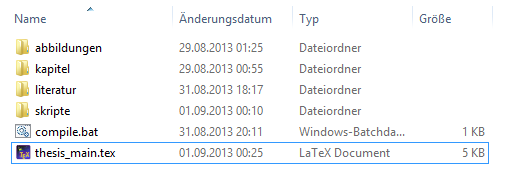
\includegraphics[width=0.9\textwidth]{verzeichnisStruktur}
\\
Quelle: Eigene Darstellung
\end{figure}

\subsection{Research Aim} \label{aim}
This paper aims to investigate the performance disparity between Web Assembly (WASM) and JavaScript (JS) in the context of client-side applications, with a focus on computationally intensive algorithms. The objective is to determine whether WASM provides a distinct advantage over JS in terms of efficiency through comprehensive experimentation and analysis.
\subsection{Research Objectives} \label{objectives}
In order to completely cover the most important topics and to have a clear outline for the research process, we defined the following research objectives:

\begin{itemize}
    \item Evaluate the performance of Web Assembly and JavaScript implementations in executing computationally intensive algorithms within client-side applications.
    \item Measure and compare CPU utilization between WASM and JavaScript implementations across various benchmark tests.
    \item Assess memory usage and management efficiency between WASM and JavaScript for tasks involving computationally intensive operations.
    \item Analyze the impact of DOM manipulation on the overall performance of WASM and JavaScript implementations within the context of client-side applications.
    \item Provide empirical evidence and insights to ascertain whether Web Assembly is advantageous over JavaScript from an efficiency perspective in the targeted application domain.
    \item Offer recommendations and guidelines for developers based on the findings to optimize performance when selecting between Web Assembly and JavaScript for client-side applications with computationally intensive algorithms.
\end{itemize}
\newpage

\section{Grundlagen} \label{grundlagen}

\subsection{Überblick der eingesetzten Technologien} \label{eingestzeTechnologien}
\subsubsection{React} \label{react}
React ist das von uns bevorzugte Frontend. Im Folgenden werden wir erklären, was React ist und wie es grundsätzlich aufgebaut ist.
React wurde von Facebook entwickelt und ist eine leistungsstarke Open-Source-Bibliothek, basierend auf JavaScript. Dabei ist React auf die Erstellung von Benutzeroberflächen, also auf das sogenannte Frontend, spezialisiert\footcite{acharya_15_2023}. Darüber hinaus ist React eine komponentenbasierte Bibliothek, welche einen effizienten und strukturierten Ansatz zur Gestaltung von interaktiven Benutzeroberflächen bietet\footcite{p_was_2024}. 
Aus diesen Gründen eignet sich die Bibliothek hervorragend für komplexe Benutzeroberflächen, welche eben aus diesen kleinen und modularen Komponenten bestehen. Für die Benutzer bedeutet der Einsatz von React anwenderfreundliche Oberflächen und für die Entwickler eine verbesserte Code-Organisation, was unter anderem zu einer erleichterten Wartung führt\footcite{laurent_komponentenbasierte_2023}.
Zudem verwendet React ein virtuelles Document Object Model (DOM). Das virtuelle DOM ist ähnlich zum tatsächlichen DOM. Es ist allerdings wesentlich leichtgewichtiger und wird als JavaScript-Objekt dargestellt. Auf Grund der Darstellung als JavaScript-Objekt werden lediglich die wirklich notwendigen Änderungen am tatsächlichen DOM durchgeführt, wodurch wiederum die Performance optimiert wird\footcite{chauhan_mastering_2023}.
React Komponenten verwenden grundsätzlich zwei verschiedene Konzepte zur Datenverwaltung. Diese beiden Konzepte nennen sich States und Props und arbeiten im Zusammenspiel, um dynamische und interaktive Benutzeroberflächen zu erstellen\footcite{bhimani_react_2024}.
States repräsentieren den internen Zustand einer Komponente und können sich im Laufe der Zeit verändern. Sie werden von der React Komponente selber verwaltet und können sowohl durch Benutzeraktionen als auch durch interne Ereignisse verändert werden\footcite{nestorowicz_state_2021}. Dies ermöglicht überhaupt erst die interaktive Nutzung der Webseite im laufenden Betrieb.
Props dagegen sind als Kurzform für Properties, zu Deutsch Eigenschaften, zu verstehen und sind unveränderlich. Sie dienen dazu, bestimmte Funktionen und Daten von einer sogenannten Elternkomponente an andere Komponenten zu übertragen\footcite{platforms_state_nodate}.
\subsubsection{Strapi} \label{strapi}
Als nächstes gehen wir auf unsere verwendete Backendstruktur ein. Die von uns gewählte Backend Technologie, nennt sich Strapi.
Strapi ist ein Headless Content Management System (CMS), das Open-Source betrieben wird. Strapi zeichnet sich durch seine Flexibilität und durch seine Entwicklerfreundlichkeit aus. Die Idee hinter Strapi ist die Trennung der Inhaltsverwaltung vom Frontend\vglfootcite{autor_strapi_2024}.
Es ermöglicht eine effiziente Erstellung, Verwaltung und Bereitstellung der Inhalte über eine integrierte und benutzerfreundliche Oberfläche. Der Headless-CMS-Ansatz bedeutet, dass alle Inhalte von der Präsentationsschicht getrennt sind. Alle Daten die in Strapi abgelegt und verwaltet werden, werden per API an das Frontend bereitgestellt\vglfootcite{behrens_headless-cms_nodate}.
Durch die Bereitstellung der Daten per API, ist Strapi in der Wahl des Frontends flexibel, da APIs grundsätzlich einem standardisierten Format folgen und jeweils leicht angepasst werden können. 
Im Folgenden werde ich etwas konkreter auf die einzelnen Vorteile von Strapi eingehen.
Ein wichtiger Aspekt von Strapi ist die vorhandene Flexibilität. Strapi ermöglicht es, Inhalte und Strukturen präzise an die eigenen Projektanforderungen anzupassen. Dabei erlaubt es die No-Code-Konfiguration, das Backend nahezu ohne eigene Programmierung einzurichten. Durch die mitgelieferte, grafische Benutzeroberfläche, können sowohl Datenfelder und Inhaltstypen als auch Relationen zwischen den Daten bequem erstellt werden\vglfootcite{viehmann_headless_2024}.
In diesem Zusammenhang ist die einfache Integration von Strapi in das Gesamtprojekt zu erwähnen. Es können unterschiedlichste Datenbanksysteme mit Strapi genutzt werden. Darunter SQL-basierte, aber auch NoSQL-basierte. Die Daten wiederum können ganz einfach per API an das unabhängige Frontend übermittelt werden\vglfootcite{autor_strapi_nodate}.
Ein weiterer äußerst wichtiger Aspekt, der von Strapi abgedeckt wird, ist die IT-Sicherheit. Strapi verfügt bereits von Haus aus, über grundlegende Sicherheitsfunktionen wie Authentifizierung und Authorisierung. Zudem liefert Strapi die Möglichkeit zur Konfiguration von Rollen- und Berechtigungskonzepten direkt mit\vglfootcite{siever_basics_2024}.
\subsubsection{JavaScript, HTML und CSS} \label{javaHtmlCss}
Neben dem eigentlichen Front- und Backend, gibt es weitere Programmiersprachen, die bei der Entwicklung einer Webseite eine Rolle spielen. In diesem Kapitel gehen wir genauer auf diese Sprachen und deren Funktionen ein.

JavaScript ist eine diversifizierte und leistungsfähige Programmiersprache, die in vielen Webentwicklungen eine Rolle spielt. JavaScript wird dabei clientseitig, also lokal auf dem jeweiligen Endgerät des Nutzers, ausgeführt. Dies ermöglicht unter Anderem den Einsatz von clientseitiger Validierung, wodurch Daten bereits lokal überprüft und somit die Serverlast reduziert werden kann\vglfootcite{sikora_professionelles_nodate}.
Der Einsatz von JavaScript ermöglicht außerdem die Implementierung von Logik und Interaktivität, wodurch die dynamischen Benutzeroberflächen im Frontend erst geschaffen und funktional gestaltet werden können. Konkret wird mit JavaScript die Manipulation des DOM ermöglicht\vglfootcite{autor_funktionen_nodate}.
Darüber hinaus können mithilfe von JavaScript Benutzerinteraktionen wie Klicks, Tastatureingaben oder Mausbewegungen verarbeitet werden. Durch den gleichzeitigen Einsatz von AJAX-Technologien können Daten asynchron mit dem Server ausgetauscht werden, wodurch die nahtlose Aktualisierung von Webseiteninhalten  und eine echte und dynamische Interaktivität sichergestellt wird\vglfootcite{autor_javascript_nodate}.
Die grundsätzliche Konzeption von JavaScript sieht vor, dass wiederverwendbare Funktionen als Kernbaustein genutzt und bei Bedarf aufgerufen werden. JavaScript unterstützt verschiedene, gängige Datentypen wie Zahlen, Zeichenketten und Objekte. Dadurch ist es auch möglich, einen objektorientierten Ansatz zu verfolgen.

Auch HTML spielt bei der Entwicklung von modernen Webseiten eine Rolle. Über HTML wird die grundlegende Strukturierung der Benutzeroberfläche vorgenommen.
Anders als bei klassischen Webseiten, wird diese Strukturierung allerdings in JavaScript XML (JSX), eine Syntaxerweiterung für JavaScript, vorgenommen.
JSX ermöglicht es Entwicklern, HTML-artige Elemente direkt in JavaScript umzusetzen, ohne explizite HTML-Syntax zu nutzen\vglfootcite{w3schools_react_nodate}.

Bei Cascading Style Sheets (CSS) handelt es sich um eine deklarative Sprache, die es ermöglicht Webseiten und deren HTML-Elemente visuell zu gestalten. Dabei gibt es verschiedene Ansätze und Möglichkeiten, wie CSS implementiert und verwaltet wird.
Zum einen gibt es die klassische CSS-Variante, bei der eine separate .css-Datei erstellt wird. In dieser Datei werden alle Styles für die Webseite definiert, was bei größeren Projekten allerdings zu Problemen bei der Wartbarkeit führen kann\vglfootcite{autor_welche_2019}.
Eine weitere Möglichkeit bieten CSS Module, die beliebig oft wiederverwendet werden können.
Die dritte Möglichkeit bieten CSS Frameworks. In diesem Fall handelt es sich um vorgefertigte Komponenten und Stile, die ebenfalls wiederverwendet werden können. Auch hier gibt es wieder verschiedene Frameworks wie zum Beispiel Bootstrap, Tailwind CSS oder Foundation.
\subsubsection{Docker} \label{docker}
Docker ist eine Open-Source-Plattform, welche zur Entwicklung, Bereitstellung und Ausführung von Anwendungen in isolierten und sogenannten Containern dient. Ein Container wiederum basiert auf einer standardisierten Einheit von Software, der alle benötigten Abhängigkeiten, Bibliotheken und Konfigurationen in einem sogenannten Image kapselt. Dadurch wird eine unabhängige Ausführung der in dem Container befindlichen Software ermöglicht, egal in welcher Umgebung sich dieser Container gerade verbindet.
Die wichtigsten Komponenten von Docker umfassen das beschriebene Docker Image, den Docker Container – einer laufenden Instanz des erstellten Imgages – und der Dockerfile bestehend aus Anweisungen zum erstellen des Docker Images\vglfootcite{beck_lokale_2023}.

\subsection{Zusammenspiel der Technologien} \label{zusammenspiel}
Für eine funktionsfähige und moderne Webseite ist das Zusammenspiel der zuvor genannten Technologien unerlässlich. Für unser Projekt bilden die klare Trennung von Backend und Frontend sowie die Integration von HTML, CSS und JavaScript, das grundlegende Fundament.

Auf Grund der genannten klaren Trennung von Frontend und Backend, können die Arbeiten an den beiden Teilprojekten unabhängig voneinander und parallel stattfinden. Außerdem bewirkt die Trennung eine gewisse Flexibilität, da Änderungen in einem der beiden Bereiche, nur geringe Auswirkungen auf den anderen Bereich haben. Darüber hinaus können beide Bereiche ebenfalls unabhängig voneinander erweitert oder skaliert werden.
Die Kommunikation zwischen den beiden Bereichen erfolgt über RESTFUL APIs. Diese APIs werden von Strapi im Backend automatisch generiert und von React im Frontend genutzt. Durch diese Vorgehensweise wird eine effiziente Datenverwaltung ermöglicht. Strapi verwaltet die Inhalte und React präsentiert sie. Die in Strapi gespeicherten Inhalte können dabei mehrfach von React im Frontend wiederverwendet werden.
HTML per JSX, CSS und JavaScript müssen im Gesamtkontext eingegliedert werden. HTML wird in React per JSX umgesetzt, um die Arbeit für Entwickler zu vereinfachen und um die grundlegende Webseitenstruktur zu bauen. CSS setzt an dem Punkt an, an dem das Design angepasst und verfeinert wird, um eine anschauliche Benutzeroberfläche zu bauen. JavaScript ist das Bindeglied zwischen den verschiedenen Technologien. Insbesondere in Form von React, wird per JavaScript der Datenfluss und die dynamische Aktualisierung der Benutzeroberfläche logisch umgesetzt und verwaltet.
Docker fungiert hier als Isolation für die ausgeführten Komponenten. Sowohl das Backend als auch das Frontend sollen innerhalb der einzelnen Container laufen.
\subsection{Vorteile der gewählten Architektur} \label{vorteile}
Im Folgenden werden die Vorteile unserer gewählten Struktur und Technologien hervorgehoben.

Ein Vorteil von der von uns gewählten Struktur, ist die Modularität und Wiederverwendbarkeit. Diese wird vor allem durch die Trennung von Front- und Backend erreicht. Hinzu kommt die Verwendung einzelner Komponenten innerhalb von React, wodurch Wartung und Erweiterung der Webseite verbessert werden\footcite{acharya_15_2023}.

Darüber hinaus ist, ebenfalls durch die Trennung von Front- und Backend, aber auch durch die Nutzung von Strapi als headless CMS, eine hohe Flexibilität bei der Entwicklung gegeben. Dadurch kann jederzeit auf äußere Einflüsse wie neue Technologien oder Kundenanforderungen eingegangen werden\footcite{autor_warum_nodate}.

Die Verwendung von APIs für den Datenfluss zwischen Front- und Backend, bietet den Vorteil, dass dieser effizient und standardisiert ablaufen kann. Strapi stellt die standardisierten APIs bereit und React greift darüber auf die benötigten und wiederverwendbaren Daten zu\footcite{autor_headless-cms_nodate}.

Strapi bietet zudem einen großen Vorteil in Sachen Sicherheit. Die integrierten Sicherheitsfunktionen in Strapi schützen das Backend und im Frontend können unabhängig davon weitere Sicherheitsmaßnahmen gezielt getroffen werden.



\newpage

\section{Hauptteil} \label{hauptteil}
Einleitende Worte zum Hauptteil.
\subsection{Architektur} \label{architektur}
Server
Frontend API Backend
Shopify

\begin{figure}[H]
    \centering
    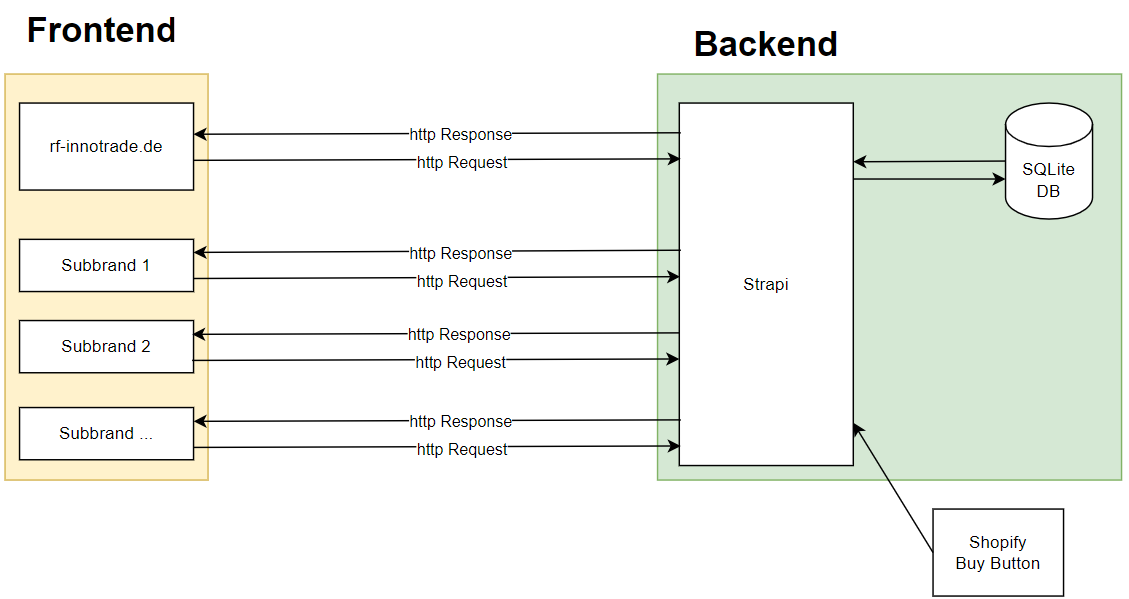
\includegraphics[width=1\textwidth]{figures/architektur.png}
    \caption{Architektur Schaubild, Quelle: Eigene Darstellung}
	\label{fig:architekturSchaubild}
\end{figure}

\subsection{Strapi als Backend} \label{strapiMain}
Strapi bietet von Haus aus eine gute Grundstruktur. Alle notwendigen Dateien werden von Strapi grundlegend mitgeliefert und müssen im Anschluss nur noch an die individuellen Anforderungen angepasst werden. In diesem Kapitel werden wir auf die von uns veränderten und auf unsere Bedürfnisse zugeschnittenen Dateien eingehen und deren Funktionalitäten erläutern.
\subsubsection{Vite.config.js} \label{viteconfigjs}
Diese Datei ist abgelegt unter: „rfinnotrade/strapi/src/admin/vite.config.js“.
Um zu erläutern, was in dieser Datei passiert, muss das grundlegende Prinzip von Cross-Origin Ressource Sharing (CORS) verstanden werden. CORS ist ein Sicherheitsmechanismus, welcher in Webbrowsern verwendet werden kann, um Zugriff auf Ressourcen von einer anderen Domain kontrolliert zulassen zu können. Daher auch der Begriff „Cross-Origin“. Es handelt sich hierbei um eine Erweiterung der standardmäßig verwendeten Same-Origin-Policy (SOP), welche Zugriffe nur von der selben Domain zulässt (Vgl. Cross-Origin Resource Sharing – Wikipedia, o. J.). In unserem Fall erlaubt diese Struktur also den Fremdzugriff auf Ressourcen innerhalb von Strapi.
Diese Datei wird ebenfalls grundsätzlich von Strapi mitgeliefert und wurde von uns leicht angepasst.

\begin{lstlisting}[language=JavaScript, caption={Vite.config.js}, label={lst:viteconfigjs}]
const { mergeConfig } = require('vite');

module.exports = (config) => {
  // Important: always return the modified config
  return mergeConfig(config, {
    resolve: {
      alias: {
        '@': '/src',
      },
    },
    server: {
      cors: {
        origin: true,
        credentials: true,
      },
    },
  });
};
\end{lstlisting}

In Zeile 13 und 14 erlauben wir den Zugriff auf Strapi und legen zudem fest, dass credentials weitergeleitet werden sollen. Hier könnte man auch weitere Restriktionen vornehmen, was von uns allerdings in der Datei „Middleware.js“ vorgenommen wurde.
\subsubsection{Middlewares.js} \label{middlewares}
Diese Datei liegt unter „rfinnotrade/strapi/config/middleware.js“.
Der Begriff Middleware in unserem Webprojekt ist als eine Softwareschicht zwischen unserer Webanwendung und dem Server zu verstehen. Die Middleware verarbeitet dabei eingehende Anfragen und ausgehende Antworten, um zum Beispiel Login- und Authentifizierungsfunktionen zu ermöglichen.
HIER CODE EINFÜGEN
Die hier gezeigte Middleware.js, arbeitet die aufgeführten Middleware-Funktionen nacheinander und in genau dieser Reihenfolge ab. Somit wird sichergestellt, dass aufeinander aufbauende Funktionen auch in der richtigen Reihenfolge ausgeführt werden. Es ist außerdem noch wichtig zu erwähnen, dass dies Strapi Middleware-Funktionen sind, da wir uns nach wie vor innerhalb unserer Strapi Konfiguration befinden.
Neben der Anmeldung unter unserer rf-innotrade.de Admin Seite oder für andere API-Calls, welche nur von einem angemeldeten Admin durchgeführt werden dürfen, ist diese Datei für die im vorherigen Kapitel erwähnte CORS-Konfiguration zuständig.
HIER CODE EINFÜGEN, ZEILE 6-16
Diese Konfiguration sorgt dafür, dass Authentifizierungsanfragen immer nur über die in Zeile 9 genannten Domains erlaubt sind und die Anfrage nur dann weiterverarbeitet werden darf.

\subsubsection{Token.js} \label{token}
Die nächste Datei ist unter dem Pfad „rfinnotrade/strapi/src/middlewares/Token.js“ abgelegt.
Diese Datei ist ebenfalls sehr wichtig, da Strapi von Haus aus keine Cookies verarbeiten kann. Die Verarbeitung von Cookies ist in unserem Fall notwendig, damit Informationen wie der aktuelle Login-Status oder welcher User, mit welchen Berechtigungen, startet gerade eine Anfrage an Strapi, abgefragt werden können.
HIER CODE EINFÜGEN
Realisiert wird diese Funktion im ersten Schritt durch das Auslesen des Cookies aus dem mitgelieferten Gesamtkontext der Webseite in Zeile 2 und 3. Im nächsten Schritt wird in den Zeilen 6 bis 8 der JSON Web Token (JWT) extrahiert. Sollte die Abfrage für ein JWT erfolgreich sein, wird in Zeile 9 und 10 das Token um „Bearer“ erweitert und dem „Authorization-Header“ des Webseitenkontextes wieder hinzugefügt.
Durch diese Middleware Funktion versteht Strapi, ob ein User berechtigter Weise eingeloggt ist oder Serveranfragen durchführen darf.
\subsubsection{Custom.js} \label{custom}
Die nachfolgende Datei liegt unter „rfinnotrade/strapi/src/api/custom/controllers/custom.js“ und beinhaltet verschiedene Funktionen. Im Folgenden werde ich auf die Funktionen „login“, „logout“ und „checkAuthStatus“ eingehen, da diese im Kontext von Strapi und den bisher genannten Funktionen am relevantesten sind.

Als erstes gehen wir auf die Login-Funktion ein. Diese Funktion erledigt die Aufgabe, den eigentlichen Login bei einer Login-Anfrage von der Admin Seite zu verifizieren, Daten aus Strapi abzufragen und darüber hinaus alle notwendigen Daten in den Cookies zu setzen.

\begin{lstlisting}[language=JavaScript, caption={Login-Funktion}, label={lst:customjsLogin}]
async login(ctx) {
    const { body } = ctx.request;
    const hostname = "localhost";
    const absoluteURL = `http://${hostname}:${strapi.config.server.port}`;
    const sanitizeOutput = (user) => {
      const {
        password,
        resetPasswordToken,
        confirmationToken,
        ...sanitizedUser
      } = user; // be careful, you need to omit other private attributes yourself
      return sanitizedUser;
    };
    try {
      console.log("Tryin to login");
      // Now submit the credentials to Strapi's default login endpoint
      let { data } = await axios.post(`${absoluteURL}/api/auth/local`, body);
      const populatedUser = await strapi.entityService.findOne(
        "plugin::users-permissions.user",
        data.user.id,
        {
          populate: {
            role: {
              fields: ["type"],
            },
          },
        }
      );
      data.user = sanitizeOutput(populatedUser);
      // Set the secure cookie
      if (data && data.jwt) {
        ctx.cookies.set("jwt", data.jwt, {
          httpOnly: true,
          secure: false,
          SameSite: "None",
          maxAge: 1000 * 60 * 60 * 24 * 7, // 7 Day Age
        });
      }
      // Respond with the jwt + user data, but now this response also sets the JWT as a secure cookie
      return ctx.send(data);
    } catch (error) {
      console.log("An error occurred:", error.response);
      return ctx.badRequest(null, error);
    }
  },
\end{lstlisting}

Um diesen Vorgang zu realisieren, wird erneut der gesamte Webseitenkontext in Zeile 1 übergeben und daraus alle „request“-Daten in Zeile 2 geladen. Hier sind unter anderem die Eingaben des Benutzers gespeichert.
Von Zeile 5 bis Zeile 13, wird die Funktion „sanitizeOutput“ deklariert, welche erst später angewendet wird.
Ab Zeile 14 wird versucht mithilfe der übergebenen Login-Daten, eine Anfrage an Strapis eigentliche Login API durchzuführen. Ist diese Anfrage erfolgreich, werden die entsprechenden Benutzerdaten aus der Strapi Datenbank geladen, unter anderem die Benutzerrollen abgefragt.
Ist alles erledigt, wird eine Cookie mit allen notwendigen Informationen zurückgegeben und in den Webseitenkontext geladen.
Somit wurde die Login Abfrage erfolgreich über eine API durchgeführt und alle notwendigen Login Informationen anschließend in den Cookies der Webseite für weiter Abfragen gespeichert. Eine automatische Logout Funktion wurde in Zeile 68 ebenfalls großzügig implementiert. Diese würde spätestens nach 7 Tagen greifen, das Cookie auslaufen und der Logout somit automatisch erfolgen.

Der ebenfalls implementierten Logout-Funktion wird zu Beginn erneut der Webseitenkontext übergeben.

\begin{lstlisting}[language=JavaScript, caption={Logout-Funktion}, label={lst:customjsLogout}]
async logout(ctx) {
    try {
      // Clear the JWT cookie
      ctx.cookies.set('jwt', null, {
        httpOnly: true,
        secure: false,
        maxAge: 0,
      });
      
      return ctx.send({
        message: 'Successfully logged out',
      });
    } catch (error) {
      return ctx.badRequest(null, error);
    }
  },
\end{lstlisting}

In Zeile 4 wird dann zunächst das Cookie aus dem Kontext ausgelesen und und das JWT auf „NULL“ gesetzt, wodurch der Logout theoretisch bereits erfolgt ist. Zusätzlich wird der automatische Logout, welcher in der Login Funktion auf 7 Tage gesetzt wird, auf den Wert 0 gesetzt.
Dadurch löst sich das Cookie selber auf und der Logout würde ebenfalls erfolgen. Das Cookie wird am Ende wieder an den Webseitenkontext zurückgegeben.

Die Funktion checkAuthStauts hat die Aufgabe, den aktuellen Login Status bei Aufruf dieser Funktion abzufragen. Diese Funktion ergänzt die Login- und Logout-Funktion also um eine weiter wichtige Funktionalität.
Die Funktion ist ähnlich aufgebaut wie Login und Logout.

\begin{lstlisting}[language=JavaScript, caption={checkAuthStatus-Funktion}, label={lst:customjsCheckAuthStatus}]
async checkAuthStatus(ctx) {
    // Check for JWT in cookies first
    const jwtCookie = ctx.cookies.get('jwt');
    
    if (!jwtCookie) {
      return ctx.unauthorized('No JWT cookie found');
    }

    try {
      const decoded = verify(jwtCookie, strapi.config.get('plugin::users-permissions.jwtSecret'));
      return ctx.send({ isAuthenticated: true, user: decoded });
    } catch (err) {
      return ctx.unauthorized('Invalid token');
    }
  },
\end{lstlisting}

Diese Funktion überprüft zunächst, ob überhaupt ein JWT vorhanden ist. Sollte das nicht so sein, wird die Anfrage abgelehnt, da kein aktueller Login erfolgt ist. Sollte ein JWT vorhanden sein, wird dieses erneut verifiziert und der Benutzer kann, entsprechend seinen Berechtigungen, Anfragen durchführen.

\subsection{React als Frontend} \label{reactFrontend}
React bildet das Herzstück unseres Frontends und ermöglicht die Erstellung einer dynamischen und interaktiven Benutzeroberfläche. In den folgenden Abschnitten werden wir die wichtigsten React-Komponenten unseres Projekts genauer betrachten und ihre Funktionen erläutern.
\subsubsection{App.jsx} \label{app}
Betrachten wir als nächstes unser Frontend. Die Hauptkomponente im Frontend ist die Datei App.jsx unter „rfinnotrade/frontend/src/App.jsx“. Diese Datei organisiert die gesamte Struktur der Webseite, steuert die Navigation und verwaltet darüber hinaus auch, in Verbindung mit den Backendkomponenten, den aktuellen Authentifizierungsstatus des Benutzers.
HIER CODE EINFÜGEN, ZEILE 45 bis 63
Der „Router“ Bereich wird verwendet, um die Navigation zwischen verschiedenen Seiten zu ermöglichen. Die Routes innerhalb dieser Sektion definieren die konkret verfügbaren Seiten.
Außerdem ist hier die Sidebar- und Header-Steuerung zu finden. Der aktuelle Zustand der Sidebar wird über „isOpen“ gesteuert und über die „toggleSidebar“ Funktion, kann zwischen den Zuständen der Sidebar gewechselt werden.
HIER CODE EINFÜGEN, ZEILE 20 bis 43
Außerdem wird in Zeile 21 ein state „isAuthenticated“, also ein veränderbarer Zustand, erzeugt und mit false initialisiert. Dazu gehört die checkAuth Funktion, welche eine Anfrage an Strapi ins Backend zur Authentifizierungsüberprüfung sendet. Diese Funktion wird bei jedem Neuladen der Seite automatisch über die ebenfalls implementiert Funktion useEffect aufgerufen.
Sollte der Nutzer abgemeldet werden oder für gewisse Funktionen der Webanwendung nicht freigeschaltet sein, wird über die hier implementierten Funktionen die Authentifizierung stets überprüft und in diesem Fall auf False gesetzt.
Die App.jsx Datei kommt immer beim Laden der Webseite zum Einsatz. Darüber hinaus wird sie genutzt, wenn der Benutzer zwischen verschiedenen Seiten der Webandwendung navigiert, damit die jeweiligen Komponenten auch geladen werden. Damit der Benutzer auch nur auf jene Bereiche und Komponenten zugreifen kann, auf die er auch zugreifen darf, sind die Authentifizierungsfunktionen implementiert.
\subsubsection{Login.jsx} \label{login}
Eine Seite, bzw. Komponente ist die Login Seite, welche unter „rfinnotrade/frontend/src/components/pages/Login.jsx“ abgelegt ist.
Die Login.jsx Datei definiert die Login Seite unseres Frontends. Sie hat grundsätzlich die Funktion, den Benutzern die Anmeldung per E-Mail oder Benutzernamen mit dem dazugehörigen Passwort zu ermöglichen.

\begin{lstlisting}[language=JavaScript, caption={Login.jsx Frontendaufbau}, label={lst:loginjsxUI}]
return (
    <div className="login-container">
            <div className="login-header">
            <h1 className="login-title">RF InnoTrade Admin Center</h1>
        </div>
        <div className="login-background">
            <div className="login-box">
                <h2 className="welcome-back">Welcome Back</h2>
                <p className="instructions">Gib deine Zugangsdaten ein, um Zugang zu deinem Account zu erhalten</p>
                <form onSubmit={handleSubmit} className="login-form">
                    <div className="form-group">
                        <input
                            type="text"
                            placeholder="Gib deine Email oder Username ein"
                            value={identifier}
                            onChange={(e) => setIdentifier(e.target.value)}
                            required
                            className="form-input"
                        />
                    </div>
                    <div className="form-group">
                        <input
                            type="password"
                            placeholder="Gib dein Passwort ein"
                            value={password}
                            onChange={(e) => setPassword(e.target.value)}
                            required
                            className="form-input"
                        />
                    </div>
                    <button type="submit" className="login-button">Anmelden</button>
                </form>
                <p className="reset-password">
                    Passwort vergessen? 
                    {/* <Link to="/password-reset">Passwort zurücksetzen </Link> */}
                </p>
                {error && <p className="login-error">{error}</p>}
            </div>
        </div>
    </div>
);
\end{lstlisting}

Das User-Interface (UI) ist ebenfalls hier implentiert und besteht aus einem Eingabefeld für die E-Mail und den Benutzernamen, einem Eingabefeld für das Passwort und einer Schaltfläche zum Absenden der Login-Daten. Wenn der Login fehlschlät, erscheint eine Fehlermeldung unterhalb des Formulars.
Das Styling der Seite wird über eine ausgelagerte Login.css Datei gesteuert.
Um den Login eines Benutzers durchzuführen, werden in der Login Komponente verschiedene Informationen verwaltet

\begin{lstlisting}[language=JavaScript, caption={Login.jsx states}, label={lst:loginjsxStates}]
const [password, setPassword] = useState('');
const [identifier, setIdentifier] = useState('');
const [error, setError] = useState('');
\end{lstlisting}

Wie hier zu sehen ist, verwaltet die Login Komponente password, identifiert und error, um die Logindaten oder Fehler bei der Anmeldung innerhalb der Komponente zu speichern und verarbeiten zu können.
Sendet der Benutzer den Login per Schaltfläche ab, wird die Funktion „handleSubmit“ aufgerufen. Diese sendet einen POST-Request an die Login-API von Strapi, überprüft dort die Anmeldedaten und der Benutzer wird bei erfolg an die Admin-Seite der Webseite weitergeleitet.

\begin{lstlisting}[language=JavaScript, caption={Login.jsx Login-Funktion}, label={lst:loginjsxLoginFunktion}]
try {
    const response = await axios.post(import.meta.env.VITE_STRAPI_BASE_URL+'api/auth/login', {
        identifier,
        password,
    }, {
        withCredentials: true // This is important for including cookies in the request
    });
    console.log('User profile', response.data.user);
    navigate('/Admin-Center'); // Redirect to the home page
    props.onLoginSuccess();
    } catch (error) {
    setError('Login fehlgeschlagen bitte überprüfe deine Eingabe.');
    }
\end{lstlisting}

Außerdem wird die Funktion „onLoginSuccess“ ausgeführt, damit der Authentifizierungsstatus des Benutzers aktualisiert wird.
\subsubsection{Sidebar.jsx} \label{sidebar}
Die Sidebar ist der Dreh- und Angelpunkt um auf der Webseite zu anderen Komponenten zu navigieren und ist unter „rfinnotrade/frontend/src/components/Sidebar.jsx“ abgelegt.
Die Sidebar enthält Links zu den anderen Seiten der Anwendung und bietet eine interaktive Funktion, um ein- und ausgeblendet zu werden.

\begin{lstlisting}[language=JavaScript, caption={Sidebar.jsx}, label={lst:sidebarjsx}]
const Sidebar = ({ isOpen, toggleSidebar }) => {

return (
    <>
    <div className={`menu-icon ${isOpen ? 'open' : ''}`} onClick={toggleSidebar}>
        <span className="menu-icon-bar"></span>
        <span className="menu-icon-bar"></span>
        <span className="menu-icon-bar"></span>
    </div>

    <div className={`sidebar ${isOpen ? 'open' : ''}`}>
        <ul className="sidebar-links">
        <li>
            <Link to="/" onClick={toggleSidebar}>Home</Link>
        </li>
        <li>
            <Link to="/brands" onClick={toggleSidebar}>Our Brands</Link>
        </li>
        <li>
            <Link to="/about" onClick={toggleSidebar}>About Us</Link>
        </li>
        <li>
            <Link to="/impressum" onClick={toggleSidebar}>Impressum</Link>
        </li>
        <li>
            <Link to="/agb" onClick={toggleSidebar}>AGB</Link>
        </li>  
        <li>
            <Link to="/kontakt" onClick={toggleSidebar}>Kontakt</Link>
        </li>

        <div className="divider"></div>
        <div className="login-section">
            <ul>
            <Link to="/admin-center" onClick={toggleSidebar}>Admin Center</Link>
            </ul>
        </div>
        </ul>
    </div>
    </>
);
};
\end{lstlisting}

Über die von der Elternkomponente „App.jsx“ übergebene isOpen-Eigenschaft, wird die sidebar grundlegend gesteuert. Die Funktion togglesidbar wird dabei jedes Mal aufgerufen, wenn der Benutzer auf das Sidebarsymbol oder einen Link innerhalb der Sidebar klickt. Mit jedem Aufruf der Funktion, wird die Sidebar dann geöffnet oder geschlossen.
\subsubsection{AdminCenter} \label{admincenter}
Als nächstes gehen wir auf das Admin-Center ein, welches unter „rfinnotrade/frontend/src/components/pages/admincenter.jsx“ gespeichert ist. Die Admin-Center Komponente stellt das Hauptverwaltungscenter für die Brands dar. Hier können neue Seiten erstellt, Seiteninhalte bearbeitet und laufende Docker-Container kontrolliert werden.
Auch diese Komponente nutzt wieder verschiedene States.

\begin{lstlisting}[language=JavaScript, caption={AdminCenter.jsx states}, label={lst:admincenterjsxStates}]
function AdminCenter() {
    const [brands, setBrands] = useState([]);
    const [error, setError] = useState('');
    const [isModalOpen, setIsModalOpen] = useState(false);
    const [newPage, setNewPage] = useState({});
    const [activeContainers, setActiveContainers] = useState([]);
    const [pageFields, setPageFields] = useState({});
}
\end{lstlisting}

Brands speichert die Liste aller erstellten Brands. Der State isModalOpen steuert die Sichtbarkeit des Modals zur Erstellung von neuen Seiten und newPage speichert die Daten der neuen Seite die erstellt werden soll ab. ActiveContainers enthält die Informationen zu aktuell laufenden Docker-Containern und pageFields speichert die Felder des content-types für Seiten.
Innerhalb der Komponente sind außerdem verschiedenste Funktionen implementiert. Im Folgenden gehen wir auf drei wichtige Funktionen ein.

\begin{lstlisting}[language=JavaScript, caption={fetchBrands-Funktion}, label={lst:admincenterjsxFetchBrandsFunktion}]
const fetchBrands = async () => {
try {
    const response = await axios.get(
    `${import.meta.env.VITE_STRAPI_BASE_URL}api/pages?populate=ColorPalette`, 
    { withCredentials: true }
    );
    setBrands(response.data.data);
} catch (err) {
    setError('Failed to fetch brands');
    console.error('Error fetching brands:', err);
}
};
\end{lstlisting}

Diese Funktion ruft die Liste der Brands über eine API ab und speichert diese dann im state brands. Nach dieser Vorgehensweise funktioniert auch fetchActiveContainers, zum abrufen und speichern der laufenden Container.

\begin{lstlisting}[language=JavaScript, caption={fetchActiveContainers-Funktion}, label={lst:admincenterjsxFetchActiveContainersFunktion}]
const fetchActiveContainers = async () => {
    try {
        const response = await axios.get(
        `${import.meta.env.VITE_STRAPI_BASE_URL}api/docker/list`,
        { withCredentials: true }
        );
        setActiveContainers(response.data);
    } catch (err) {
        setError('Failed to fetch running containers');
        console.error('Error fetching running containers:', err);
    }
    };
\end{lstlisting}

In Zeile 4 ist ein beispielhafter API-Endpunkt zu sehen. Das Frontend greift über diese API auf das Backend in Strapi zu und lädt von dort aus die laufenden Docker-Container. 

\begin{lstlisting}[language=JavaScript, caption={fetchPageFields-Funktion}, label={lst:admincenterjsxFetchPageFieldsFunktion}]
const fetchPageFields = async () => {
    try {
        // Fetch the main content type
        const mainFields = await fetchContentType('api::page.page');
        if (!mainFields) return;

        // Process components recursively
        const processedFields = {};
        for (const [key, field] of Object.entries(mainFields)) {
        if (field.type === 'component') {
            // Fetch and process component fields
            const componentFields = await fetchComponent(field.component);
            processedFields[key] = {
            ...field,
            fields: componentFields
            };
        } else {
            processedFields[key] = field;
        }
        }
    }
}
\end{lstlisting}

Diese Funktion sorgt dafür, dass Felddefinitionen des Seiten-Content-Types sowie zugehörige Komponenten geladen und die Struktur der neuen Seite initialisiert werden. Dies ist also die Hauptfunktion, um die in den Feldern vom Benutzer eingetragenen Daten für die neue Seite zu übernehmen und die Initialisierung der neuen Brand zu starten.
Auch im admin-center ist wieder der eigentliche Webseitenaufbau in der html-nahen jsx-Syntax zu finden.

\begin{lstlisting}[language=JavaScript, caption={AdminCenter.jsx Aufbau}, label={lst:admincenterjsxAufbau}]
return (
    <div className="admin-center">
        <div className="brand-management">
        <div className="subheader">
            <h2 className="center-title" > Admin Center </h2>
            <button onClick={openModal} className="add-brand-btn">+ New Page</button>
        </div>
        
        {isModalOpen && (
            <div className="modal-overlay">
            <div className="modal-content">
                <h3>Neue Seite erstellen</h3>
                <form onSubmit={handleSubmit}>
                {Object.entries(pageFields).map(([key, field]) => 
                    renderField(key, field, '', newPage, setNewPage, setError)
                )}
                <div className="modal-actions">
                    <button type="button" onClick={closeModal}>Cancel</button>
                    <button type="submit">Seite erstellen</button>
                </div>
                </form>
            </div>
            </div>
        )}

        <div className="brand-list">
            {brands.map((brand, index) => {
            const isRunning = activeContainers.some(container => container.name === `subbrand-${brand.documentId}`);
            return (
                <BrandItem
                key={brand.id || index}
                name={brand.BrandName || `Brand ${index + 1}`}
                page={brand}
                refreshBrands={() => fetchBrands()}
                isRunning={isRunning}
                fetchActiveContainers={fetchActiveContainers}
                pageFields={pageFields}
                isEditing={activeEditBrandId === brand.documentId} // Check if this brand is being edited
                toggleEdit={() => toggleEditBrand(brand.documentId)} // Toggle edit mode
                />
            );
            })}
        </div>
        </div>
    </div>
    );
\end{lstlisting}

Der Aufbau der Webseite ist dabei grundsätzlich in zwei Teile unterteilt. Die eigentliche admin-center Seite und die darin integrierte brand-list.

\subsection{Subbrands} \label{subbrands}
Im Folgenden gehen wir auf den Subbrand Bereich ein. In diesem Kapitel geht es konkret um die jeweils erstellten Subbrandseiten, wobei wir hier auch teilweise auf Frontend- und Stylingelemente eingehen.
\subsection{Design} \label{design}
\input{chapter/chapter_3/design.tex}
\subsection{Docker} \label{dockermain}
Für Docker und zur Erstellung von Containern ist jeweils im Frontend, Backend und in Subbrands eine Dockerfile geschrieben, über die Docker Images erstellt werden. Alle einzelnen Komponenten laufen in einem eigens kreierten Container. Strapi im Backend, das admin Center im Frontend und auch die einzelnen Subbrands werden in einem eigenen Docker Container gestartet.
Die Container für Strapi und das Admin Center laufen jeweils automatisch und dauerhaft. Lediglich die Subbrands können über das Admin Center eigenhändig gestartet und gestoppt werden, wobei der initialie Start des Containers einer Subband immer manuell ausgeführt werden muss.

\begin{lstlisting}[language=JavaScript, caption={Middlewares.js}, label={lst:middlewaresjs}]
# Use the official Node.js image for building the React app
FROM node:alpine AS build

# Set the working directory for the build
WORKDIR /app

# Copy package.json and package-lock.json
COPY package*.json ./

# Install dependencies with increased memory limit
RUN node --max-old-space-size=2048 $(which npm) install

# Copy the rest of the application code
COPY . .
ARG VITE_DOCUMENTID
ENV VITE_DOCUMENTID=${VITE_DOCUMENTID}
ENV VITE_STRAPI_BASE_URL=http://www.rf-innotrade.de:1337
# Build the React app
RUN npm run build

# Use the official Nginx image for serving static files
FROM nginx:alpine

# Set the working directory in the container
WORKDIR /usr/share/nginx/html

# Remove the default Nginx static assets
RUN rm -rf ./*

# Copy the prebuilt React files from the build stage
COPY --from=build /app/dist /usr/share/nginx/html
COPY nginx.conf /etc/nginx/conf.d/default.conf

# Expose port 80
EXPOSE 80

# Start Nginx in the foreground
CMD ["nginx", "-g", "daemon off;"]
\end{lstlisting}

Die Dockerfile ist in einem zweistufigen Build- und Deployment-Prozess aufgebaut.
Der erste Prozess ist die Build-Phase, in der ein Node.js-Image genutzt wird, um die React-App zu bauen. Darüber hinaus werden alle notwendigen Abhängigkeiten installiert und vorallem werden die dynamischen Umgebungsvariablen gesetzt, um spezifische Subbranddaten wie Ids, oder API-URLs zu definieren. Am Ende wird die React-App gebaut und im Ordner dist abgelegt.
Der zweite Prozess ist die Deployment-Phase. Hier wird Nginx als Webserver genutzt und alle generierten Dateien aus der Build-Phase in den Nginx-Container kopiert.
Zuletzt wird der Container bereitgestellt und über Port 80 erreichbar gemacht.
Mithilfe dieser Vorgehensweise werden die einzelnen Subbrands in Container gekapselt und können trotzdem über API-Aufrufe verändert und verwaltet werden.
\newpage

\section{Empirische Analyse} \label{empirischeanalyse}
Im folgenden Kapitel wird zur Beantwortung der Forschungsfrage die empirische Untersuchung der Daten aus dem Deutschlandatlas durchgeführt. Die Daten sollen systematisch ausgewertet werden, um die Eignung für die Vorhersage von Immobilienkaufpreisen zu überprüfen. Aufbauend auf den vorherigen Kapiteln werden die einzelnen Schritte des Analyseprozesses transparent dargestellt. Damit wird sichergestellt, dass das Vorgehen nachvollziehbar ist und die Ergebnisse replizierbar sind.

\subsection{Datenbeschreibung und -aufbereitung} \label{datenbeschreibungundaufbereitung}
Claras Teil
\begin{itemize}
    \item Beschreibung der verwendeten Datensätze:
    \item Schritte der Datenbereinigung und -transformation:
    \item Zusammenführung von Deutschlandatlas- und Preisdaten (falls nötig):
\end{itemize}

\subsection{Modellierung und Feature-Importance-Analyse} \label{modellierungundfeatureimportanceanalyse}
In diesem Abschnitt wird darauf eingegangen was getan wurde um ein geeignetes Modell zu erstellen und die wichtigsten Variablen zu identifizieren, die den Immobilienkaufpreis beeinflussen. Außerdem wird afu den damiteinhergenenden Trainingsprozess eingegangen und wie die Top-10-Variablen dargestellt werden.

Nachdem die Daten in Abschnitt "Datenbeschreibung und Aufbereitung" beschrieben und aufbereitet wurden, folgt hier die eigentliche Modellierung und Analyse der Feature Importance. Ziel ist es, ein geeignetes Machine Learning (ML)-Modell zu entwickeln, das die Immobilienkaufpreise vorhersagen kann, sowie die wichtigsten Einflussfaktoren zu identifizieren.
Der erste Schritt im Programmcode ist dabei die Definierung des Trainings- und Testdatensatzes. Hierbei wird der Datensatz in zwei Teile aufgeteilt: einen Trainingsdatensatz, der für das Training des Modells verwendet wird, und einen Testdatensatz, der zur Validierung der Modellleistung dient. Dies ist wichtig, um sicherzustellen, dass das Modell generalisierbar ist und nicht nur die Trainingsdaten auswendig lernt.
Dazu wurde ein 80/20-Split verwendet, was bedeutet, dass 80\% der Daten für das Training und 20\% für den Test verwendet werden. Dies ist eine gängige Praxis im Machine Learning, um die Leistung des Modells auf unbekannten Daten zu überprüfen (Zitat?). Außerdem werden die Features mit StandardScaler skaliert uns standadisiert, um sicherzustellen, dass alle Variablen auf der gleichen Skala liegen. Es wurde ein Mittelwert von 0 und eine Varianz von 1 angezielt.

Hier Code

Der nächste Schritt ist das Modelltraining. Dies wird über die Funktion \textit{train\_improved\_models} realisiert. Dabei werden vier verschiedene Modelle trainert, um die beste Leistung zu ermitteln. Die Modelle umfassen:
\begin{itemize}
    \item Random Forest Regressor
    \item Gradient Boosting Regressor
    \item XGBoost Regressor
    \item LightGBM Regressor
\end{itemize}
Es wurde sich dazu entschieden für jedes der Modelle eine 5-fache Cross-Validation durchzuführen und die besten Hyperparameter zu ermitteln. Dies hilft, die Leistung der Modelle zu optimieren und Überanpassung zu vermeiden. Die Ergebnisse der Modelle werden in einem DataFrame gespeichert, der die mittlere absolute Fehler (MAE) und den mittleren quadratischen Fehler (MSE) für jedes Modell enthält.


Nach dem Modelltraining folgt die Visualisierung der Ergebnisse. Dies passiert in der Funktion \textit{create\_enhanced\_plots}, welche verschiedene Plots erstellt, um die Ergebnisse der Modelle anschaulich zu machen und die Modellgüte visuell überprüfen zu können.
Als Plot werden ausgegeben:
\begin{itemize}
    \item Ein Säulendiagramm, das die mittleren absoluten Fehler (MAE) der Modelle vergleicht.
    \item Ein Streudiagramm pro Modell, das die tatsächlichen Immobilienkaufpreise gegen die vorhergesagten Preise darstellt und die Güte der Vorhersage visualisiert.
    \item Ein Streudiagramm, das die Residuen (Fehler) der Modelle gegen die vorhergesagten Preise zeigt, um zu überprüfen, ob die Fehler zufällig verteilt sind.
    \item Ein Boxplot, der die Verteilung der Fehler für jedes Modell zeigt.
    \item Ein Balkendiagramm, das die Feature Importance des besten Modells darstellt, um die wichtigsten Einflussfaktoren auf die Immobilienkaufpreise zu identifizieren.
    \item Ein Balkendiagramm welches die Top 10 Variablen mit der höchsten Correlation zu den Immobilienkaufpreisen zeigt.
    \item Ein Säulendiagramm das die Fehlerverteilung des besten Modells zeigt.
    \item Ein Liniendiagramm mit Konfidenzintervallen um zu zeigen, wie gut das beste Modell die Preise vorhersagt und mit welcher Unsicherheit es das tut.
\end{itemize}

Nach der Erstellung der Plots wird das beste Modell sowie der dazugehörige Scaler mit der Bibliothek "joblib" gespeichert, um sie später für Vorhersagen verwenden zu können. 

Daraufhin wird eine Feature Importance Analyse durchgeführt, um die wichtigsten Variablen zu identifizieren, die den Immobilienkaufpreis beeinflussen. Dies ist entscheidend, um zu verstehen, welche Faktoren am stärksten mit den Preisen korrelieren und somit für die Vorhersage am relevantesten sind. Die Feature Importance wird für das am besten performende Modell berechnet und in einem DataFrame gespeichert.

Um Aussagen über Daten treffen zu können die 

\subsection{Bewertung und Interpretation} \label{bewertungundinterpretation}
\begin{itemize}
    \item Wie gut funktioniert das Modell? (z.B. Metriken wie R², RMSE)
    \item Welche Variablen sind am wichtigsten?
    \item Interpretation der wichtigsten Einflussfaktoren auf die Immobilienpreise
\end{itemize}

%-----------------------------------
% Apendix / Anhang
%-----------------------------------
\newpage
\section*{Appendices} %Überschrift "Anhang", ohne Nummerierung
\addcontentsline{toc}{section}{Appendices} %Den Anhang ohne Nummer zum Inhaltsverzeichnis hinzufügen

\begin{appendices}
	% Nachfolgende Änderungen erfolgten aufgrund von Issue 163
	\makeatletter
	\renewcommand\@seccntformat[1]{\csname the#1\endcsname:\quad}
	\makeatother
	\addtocontents{toc}{\protect\setcounter{tocdepth}{0}} %
		\renewcommand{\thesection}{\appendixname\ \arabic{section}}
		\renewcommand{\thesubsection}{\appendixname\ \arabic{section}.\arabic{subsection}}
		\section{Literature appendices}
Together with the paper, the following literature appendices are submitted:

\begin{itemize}
    \item Sunarto et al. - 2023 - A Systematic Review of WebAssembly VS Javascript P.pdf
    \item De Macedo et al. - 2022 - WebAssembly versus JavaScript Energy and Runtime.pdf
    \item javascript-issues-and-solutions.html
    \item 10-most-common-javascript-mistakes.html
    \item what-to-understand-callback-and-callback-hell-in-javascript.html
    \item introduction.html
    \item what-is-the-dom-explained-in-plain-english.html
    \item vanilla-javascript-libraries-quest-stateful-dom-rendering.html
    \item javascript-performance.html
    \item js_performance.html
    \item was-ist-ein-assembler-a-756636.html
    \item using-git-and-github-for-latex-writting.html
    \item a-git-workflow-for-writing-papers-in-latex-4cfb31be4b06.html
    \item _Einleitung.html
    \item ITInfraPaper.html
    \item WASMvsJS.html
    \item webassembly-solving-performance-problems.html
    \item experimental-design.html
    \item hitlist.html
    \item experiment.html
    \item Sieve_of_Eratosthenes.html
    \item webassembly-mehr-als-nur-ein-web-standard.html
    \item was-ist-webassembly-a-4243591d831cc5a12d425ede224f5e5b.html
    \item WebAssembly-Wasm.html
    \item javascript-vs-webassembly.html
    \item downsides-of-rust-programming-language.html
    \item rust-worlds-fastest-growing-programming-language.html
    \item 2023.html
    \item was-ist-ein-compiler.html
    \item was-ist-ein-interpreter.html
    \item Concepts.html
    \item FOM-LaTeX-Template.html
    \item Rust_to_wasm.html
\end{itemize}
They can also be found in the literature appendices folder of the GitHub repository.

\section{GitHub Repositories}
Here are the links to the GitHub repositories that contain the code and data from the \LaTeX Project used in this paper:
\begin{itemize}
    \item \href{https://github.com/nilsrueber/ITInfraPaper}{ITInfraPaper}
    \item \href{https://github.com/Foxx-l/WASMvsJS}{WASMvsJS}
\end{itemize}
	\end{appendices}
	\addtocontents{toc}{\protect\setcounter{tocdepth}{2}}

%-----------------------------------
% Literaturverzeichnis
%-----------------------------------
\newpage

% Die folgende Zeile trägt ALLE Werke aus literatur.bib in das
% Literaturverzeichnis ein, egal ob sie zietiert wurden oder nicht.
% Der Befehl ist also nur zum Test der Skripte sinnvoll und muss bei echten
% Arbeiten entfernt werden.
%\nocite{*}

%\addcontentsline{toc}{section}{Literatur}

% Die folgenden beiden Befehle würden ab dem Literaturverzeichnis wieder eine
% römische Seitennummerierung nutzen.
% Das ist nach dem Leitfaden nicht zu tun. Dort steht nur dass 'sämtliche
% Verzeichnisse VOR dem Textteil' römisch zu nummerieren sind. (vgl. S. 3)
%\pagenumbering{Roman} %Zähler wieder römisch ausgeben
%\setcounter{page}{4}  %Zähler manuell hochsetzen

% Ausgabe des Literaturverzeichnisses

% Keine Trennung der Werke im Literaturverzeichnis nach ihrer Art
% (Online/nicht-Online)
%\begin{RaggedRight}
%\printbibliography
%\end{RaggedRight}

% Alternative Darstellung, die laut Leitfaden genutzt werden sollte.
% Dazu die Zeilen auskommentieren und folgenden code verwenden:

% Literaturverzeichnis getrennt nach Nicht-Online-Werken und Online-Werken
% (Internetquellen).
% Die Option nottype=online nimmt alles, was kein Online-Werk ist.
% Die Option heading=bibintoc sorgt dafür, dass das Literaturverzeichnis im
% Inhaltsverzeichnis steht.
% Es ist übrigens auch möglich mehrere type- bzw. nottype-Optionen anzugeben, um
% noch weitere Arten von Zusammenfassungen eines Literaturverzeichnisse zu
% erzeugen.
% Beispiel: [type=book,type=article]
\printbibliography[nottype=online,heading=bibintoc,title={References}]

% neue Seite für Internetquellen-Verzeichnis
\newpage

% Laut Leitfaden 2018, S. 14, Fussnote 44 stehen die Internetquellen NICHT im
% Inhaltsverzeichnis, sondern gehören zum Literaturverzeichnis.
% Die Option heading=bibintoc würde die Internetquelle als eigenen Eintrag im
% Inhaltsverzeicnis anzeigen.
%\printbibliography[type=online,heading=bibintoc,title={\headingNameInternetSources}]
\printbibliography[type=online,heading=subbibliography,title={\headingNameInternetSources}]

\newpage
\pagenumbering{gobble} % Keine Seitenzahlen mehr

%-----------------------------------
% Ehrenwörtliche Erklärung
%-----------------------------------
\section*{Eigenständigkeitserklärung}

\noindent Hiermit versichere ich, dass ich die angemeldete Prüfungsleistung in allen Teilen eigen\-ständig ohne Hilfe von Dritten anfertigen und keine anderen als die in der Prüfungsleis\-tung angegebenen Quellen und zugelassenen Hilfsmittel verwenden werde. Sämtliche wörtlichen und sinngemäßen Übernahmen inklusive KI-generierter Inhalte werde ich kenntlich machen. Diese Prüfungsleistung hat zum Zeitpunkt der Abgabe weder in glei\-cher noch in ähnlicher Form, auch nicht auszugsweise, bereits einer Prüfungsbehörde zur Prüfung vorgelegen; hiervon ausgenommen sind Prüfungsleistungen, für die in der Mo\-dulbeschreibung ausdrücklich andere Regelungen festgelegt sind. Mir ist bekannt, dass die Zuwiderhandlung gegen den Inhalt dieser Erklärung einen Täuschungsversuch dar\-stellt, der das Nichtbestehen der Prüfung zur Folge hat und daneben strafrechtlich gem. § 156 StGB verfolgt werden kann. Darüber hinaus ist mir bekannt, dass ich bei schwerwie\-gender Täuschung exmatrikuliert und mit einer Geldbuße bis zu 50.000 EUR nach der für mich gültigen Rahmenprüfungsordnung belegt werden kann. Ich erkläre mich damit ein\-verstanden, dass diese Prüfungsleistung zwecks Plagiatsprüfung auf die Server externer Anbieter hochgeladen werden darf. Die Plagiatsprüfung stellt keine Zurverfügungstellung für die Öffentlichkeit dar.

\vspace{2cm}

\noindent\begin{tabular}{@{}p{0.5\textwidth}@{}p{0.5\textwidth}@{}}
{\raggedleft Bonn, 06.01.25} & {\raggedright\rule{5cm}{0.4pt}} \\
& {\raggedright Unterschrift}
\end{tabular}


% \par\medskip
% \par\medskip

\vspace{5cm}

% 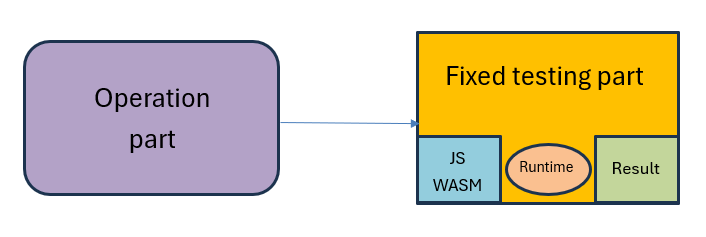
\includegraphics{signatures.png}
\end{document}
